\section{Supervised Learning without Neural Networks}
\label{sec: linear methods for supervised learning}
\textit{Supervised learning}\index{supervised learning} is the term for a machine learning task, where we are given a dataset consisting of input-output pairs $\lbrace(\bm{x}_{1}, y_{1}), \dots, (\bm{x}_{m}, y_{m})\rbrace$ and our task is to "learn" a function which maps input to output $f: \bm{x} \mapsto y$. Here we chose a vector-valued input $\bm{x}$ and only a single real number as output $y$, but in principle also the output can be vector valued. The output data that we have is called the \emph{ground truth} and sometimes also referred to as ``labels'' of the input. In contrast to supervised learning, all algorithms presented so far were unsupervised, because they just relied on input-data, without any ground truth or output data.
 
Within the scope of supervised learning, there are two main types of tasks: \textit{Classification}\index{classification} and \textit{Regression}\index{regression}. In a classification task, our output $y$ is a discrete variable corresponding to a classification category. An example of such a task would be to distinguish stars with a planetary system (exoplanets) from those without given time series of images of such objects. On the other hand, in a regression problem, the output $y$ is a continuous number or vector. For example predicting the quantity of rainfall based on meteorological data from the previous days.

In this section, we first familiarize ourselves with linear methods for achieving these tasks. Neural networks, in contrast, are a non-linear method for supervised classification and regression tasks.

\subsection{Linear regression}\label{sec:linear regression}
Linear regression, as the name suggests, simply means to fit a linear model to a dataset. Consider a dataset consisting of input-output pairs  $\lbrace(\bm{x}_{1}, y_{1}), \dots, (\bm{x}_{m}, y_{m})\rbrace$, where the inputs are $n$-component vectors $\boldsymbol{x}^{T} = (x_1, x_2, \dots , x_n)$ and the output $y$ is a real-valued number. The linear model then takes the form
\begin{equation} \label{eqn: Univariate Linear Model}
     f(\boldsymbol{x}|\bm{\beta}) = \beta_0 + \sum_{j=1}^{n} \beta_{j}x_{j} 
\end{equation}
or in matrix notation
\begin{equation}\label{eqn: Univariate Linear Model Matrix Form}
    f(\boldsymbol{x}|\bm{\beta}) = \tilde{\bm{x}}^{T}\bm{\beta}
\end{equation}
where $\bm{\tilde{x}}^{T} = (1, x_1, x_2, \dots , x_n)$ 
and $\bm{\beta} = (\beta_0, \dots, \beta_n)^{T}$ are $(n+1)$ dimensional row vectors. %The contraction of the row with column vector is implied in Eq.~\eqref{eqn: Univariate Linear Model Matrix Form}. 

The aim then is to find parameters $\hat{\bm{\beta}}$ such that $f(\bm{x}|\hat{\bm{\beta}})$ is a good \emph{estimator}\index{estimator} for the output value $y$. In order to quantify what it means to be a ``good'' estimator, one need to specify a real-valued \emph{loss function}\index{loss function} $L(\bm{\beta})$, sometimes also called a \emph{cost function}\index{cost function}. The good set of parameters $\hat{\bm{\beta}}$ is then the  minimizer of this loss function
\begin{equation}
    \hat{\bm{\beta}} = \mathop{\mathrm{argmin}}_{\bm{\beta}} L(\bm{\beta}).
\end{equation}
There are many, inequivalent, choices for this loss function. For our purpose, we choose the loss function to be \textit{residual sum of squares} (RSS) defined as
\begin{equation}\label{eqn: RSS}
\begin{split}
    \textrm{RSS}(\bm{\beta}) &= \sum_{i=1}^{m} [y_{i} -  f(\bm{x}_{i}|\bm{\beta})]^{2} \\
    &= \sum_{i=1}^{m} \left(y_{i} -  \beta_0 -\sum_{j=1}^{n} \beta_{j}x_{ij}\right)^{2},
\end{split}
\end{equation}
where the sum runs over the $m$ samples of the dataset. This loss function is sometimes also called the \emph{L2-loss} and can be seen as a measure of the distance between the output values from the dataset $y_i$ and the corresponding predictions $f(\bm{x}_i|\bm{\beta})$.

It is convenient to define the $m$ by $(n+1)$ data matrix $\widetilde{X}$, each row of which corresponds to  an input sample $\bm{\tilde{x}}^{T}_{i}$, as well as the output vector $\bm{Y}^{T} = (y_{1}, \dots, y_{m})$. With this notation, Eq.~\eqref{eqn: RSS} can be expressed succinctly as a matrix equation
\begin{equation}
    \textrm{RSS}(\bm{\beta}) = (\bm{Y} - \widetilde{X}\bm{\beta})^{T}(\bm{Y} - \widetilde{X}\bm{\beta}).
    \end{equation}
The minimum of $\textrm{RSS}(\bm{\beta})$ can be easily solved by considering the partial derivatives with respect to $\bm{\beta}$, i.e.,
\begin{equation}
\begin{split}
  &\frac{\partial \textrm{RSS}}{\partial \bm{\beta}} = -2 \widetilde{X}^{T}(\bm{Y} - \widetilde{X}\bm{\beta}), \\
  &\frac{\partial^{2} \textrm{RSS}}{\partial \bm{\beta}\partial \bm{\beta}^{T}} = 2 \widetilde{X}^{T}\widetilde{X}.
\end{split}
\end{equation}
At the minimum, $\frac{\partial \textrm{RSS}}{\partial \bm{\beta}} = 0$ and $\frac{\partial^{2} \textrm{RSS}}{\partial \bm{\beta}\partial \bm{\beta}^{T}}$ is positive-definite. Assuming $ \widetilde{X}^{T}\widetilde{X}$ is full-rank and hence invertible, we can obtain the solution $\hat{\bm{\beta}}$ as 
\begin{equation}\label{eqn: LG RSS Solution}
\begin{split}
    &\left.\frac{\partial \textrm{RSS}}{\partial \bm{\beta}}\right|_{\bm{\beta}=\hat{\bm{\beta}}} = 0, \\
      \implies &\widetilde{X}^{T}\widetilde{X}\hat{\bm{\beta}} = \widetilde{X}^{T}\bm{Y}, \\
    \implies 
 & \hat{\bm{\beta} }=  (\widetilde{X}^{T}\widetilde{X})^{-1} \widetilde{X}^{T} \bm{Y}.
\end{split}
\end{equation}
If $ \widetilde{X}^{T}\widetilde{X}$ is not full-rank, which can happen if certain data features are perfectly correlated (e.g., $x_1 = 2x_3$), the solution to $\widetilde{X}^{T}\widetilde{X}\bm{\beta} = \widetilde{X}^{T}\bm{Y}$ can still be found, but it would not be unique. Note that the RSS is not the only possible choice for the loss function and a different choice would lead to a different solution.

What we have done so far is uni-variate linear regression, that is linear regression where the output $y$ is a single real-valued number. The generalisation to the multi-variate case, where the output is a $p$-component vector $\bm{y}^{T} = (y_1, \dots y_p)$, is straightforward. The model takes the form
\begin{equation} \label{eqn: Multivariate Linear Model}
    f_{k}(\bm{x}|\beta) = \beta_{0k} + \sum_{j=1}^{n} \beta_{jk}x_{j}.
\end{equation}
where the parameters $\beta_{jk}$ now have an additional index $k = 1, \dots, p$. Considering the parameters $\beta$ as a $(n+1)$ by $p$ matrix, we can show that the solution takes the same form as before [Eq.~\eqref{eqn: LG RSS Solution}] with $Y$ as a $m$ by $p$ output matrix.


\subsubsection{Statistical analysis}
Let us stop here and evaluate the quality of the method we have just introduced. At the same time, we will take the opportunity to introduce some statistics notions, which will be useful throughout the book.

Up to now, we have made no assumptions about the dataset we are given, we simply stated that it consisted of input-output pairs, $\{(\bm{x}_{1}, y_{1}), \dots,$ $(\bm{x}_{m}, y_{m})\}$. In order to assess the accuracy of our model in a mathematically clean way, we have to make an additional assumption.
The output data $y_1\ldots, y_m$ may arise from some measurement or observation. Then, each of these values will generically be subject to errors $\epsilon_1,\cdots, \epsilon_m$ by which the values deviate from the ``true'' output without errors,
\begin{equation} \label{eqn: True Linear_b}
\begin{split}
        y_i &= y^{\textrm{true}}_i + \epsilon_i,\qquad i=1,\cdots,m.
\end{split}
\end{equation}
We assume that this error $\epsilon$ is a Gaussian random variable with mean $\mu = 0$ and variance $\sigma^2$, which we denote by $\epsilon \sim \mathcal{N}(0, \sigma^2)$. Assuming that a linear model in Eq.~\eqref{eqn: Univariate Linear Model} is a suitable model for our dataset, we are interested in the following question: How does our solution $\hat{\bm{\beta}}$ as given in Eq.~\eqref{eqn: LG RSS Solution} compare with the true solution $\bm{\beta}^{\textrm{true}}$ which obeys
\begin{equation} \label{eqn: True Linear}
\begin{split}
        y_i = \beta_0^{\textrm{true}} + \sum_{j=1}^{n} \beta_{j}^{\textrm{true}}x_{ij} + \epsilon_i,\qquad
        i=1,\ldots,m?
\end{split}
\end{equation}
  

In order to make statistical statements about this question, we have to imagine that we can fix the inputs $\bm{x}_{i}$ of our dataset  and repeatedly draw samples for our outputs $y_i$. Each time we will obtain a different value for $y_i$ following Eq.~\eqref{eqn: True Linear}, in other words the $\epsilon_i$ are uncorrelated random numbers.
%each time the value for $\epsilon_i$ is a different random number. 
This allows us to formalise the notion of an \emph{expectation value}\index{expectation value} $E(\cdots)$ as the average over an infinite number of draws. 
%For our case, we are interested in the solution $\hat{\bm{\beta}}$. 
For each draw, we obtain a new dataset, which differs from the other ones by the values of the outputs $y_i$. With each of these datasets, we obtain a different solution $\hat{\bm{\beta}}$ as given by Eq.~\eqref{eqn: LG RSS Solution}. The expectation value $E(\hat{\bm{\beta}})$ is then simply the average value we obtained across an infinite number of datasets. The deviation of this average value from the ``true'' value given perfect data is called the \emph{bias} of the model,
\begin{equation}\label{eqn: Bias}
    \textrm{Bias}(\hat{\bm{\beta}}) = E(\hat{\bm{\beta}})-\bm{\beta}^{\textrm{true}}.
\end{equation}
%A nonzero value of Eq.~\eqref{eqn: Bias} indicates that ... .

For the linear regression we study here, the bias is exactly zero, because
\begin{equation}\label{eqn: LG RSS Unbiased}
    \begin{split}
      E(\hat{\bm{\beta}}) &= E\left((\widetilde{X}^{T}\widetilde{X})^{-1} \widetilde{X}^{T} (\bm{Y}^{\textrm{true}}+\bm{\epsilon})\right)\\
      &=\bm{\beta}^{\textrm{true}},
    \end{split}
\end{equation}
where the second line follows because $E(\bm{\epsilon}) = \bm{0}$ and $(\widetilde{X}^{T}\widetilde{X})^{-1} \widetilde{X}^{T} \bm{Y}^{\textrm{true}} = \bm{\beta}^{\textrm{true}}$. Equation~\eqref{eqn: LG RSS Unbiased} implies linear regression is unbiased. Note that other machine learning algorithms will in general be biased.

What about the standard error or uncertainty of our solution? This information is contained in the \emph{covariance matrix}\index{covariance matrix}
\begin{equation}
\begin{split}
    \textrm{Var}(\hat{\bm{\beta}}) &= E\left([\hat{\bm{\beta}} - E(\hat{\bm{\beta}})][\hat{\bm{\beta}} - E(\hat{\bm{\beta}})]^{T} \right).
\end{split}
\end{equation}
The covariance matrix can be computed for the case of linear regression using the solution in Eq.~\eqref{eqn: LG RSS Solution}, the expectation value in Eq.~\eqref{eqn: LG RSS Unbiased} and the assumption in Eq.~\eqref{eqn: True Linear} that $Y = Y^{\textrm{true}} + \bm{\epsilon}$ yielding
\begin{equation}
\begin{split}
    \textrm{Var}(\hat{\bm{\beta}}) &= E\left([\hat{\bm{\beta}} - E(\hat{\bm{\beta}})][\hat{\bm{\beta}} - E(\hat{\bm{\beta}})]^{T} \right)\\
     &= E\left( \left[ (\widetilde{X}^{T}\widetilde{X})^{-1} \widetilde{X}^{T} \bm{\epsilon} \right] \left[ (\widetilde{X}^{T}\widetilde{X})^{-1} \widetilde{X}^{T} \bm{\epsilon}\right]^{T} \right) \\
    &= E\left( (\widetilde{X}^{T}\widetilde{X})^{-1} \widetilde{X}^{T} \bm{\epsilon} \bm{\epsilon}^{T} \widetilde{X} (\widetilde{X}^{T}\widetilde{X})^{-1}  \right).
\end{split}
\end{equation}
This expression can be simplified by using the fact that our input matrices $\widetilde{X}$ are independent of the draw such that
\begin{equation}
\begin{split}
\textrm{Var}(\hat{\bm{\beta}})
    &= (\widetilde{X}^{T}\widetilde{X})^{-1} \widetilde{X}^{T} E(\bm{\epsilon} \bm{\epsilon}^{T}) \widetilde{X} (\widetilde{X}^{T}\widetilde{X})^{-1} \\
    &= (\widetilde{X}^{T}\widetilde{X})^{-1} \widetilde{X}^{T} \sigma^2 I \widetilde{X} (\widetilde{X}^{T}\widetilde{X})^{-1} \\
    &= \sigma^2 (\widetilde{X}^{T}\widetilde{X})^{-1}.
\end{split}
\end{equation}
Here, the second line follows from the fact that different samples are uncorrelated, which implies that $E(\bm{\epsilon} \bm{\epsilon}^{T}) = \sigma^2 I$ with $I$ the identity matrix. The diagonal elements of $\sigma^2 (\widetilde{X}^{T}\widetilde{X})^{-1}$ then correspond to the variance\index{variance}
\begin{equation}
\begin{split}
    \textrm{Var}(\hat{\bm{\beta}}) &= E\left([\hat{\bm{\beta}} - E(\hat{\bm{\beta}})][\hat{\bm{\beta}} - E(\hat{\bm{\beta}})]^{T} \right)\\
     &= \sigma^2 (\widetilde{X}^{T}\widetilde{X})^{-1}.
\end{split}
\end{equation}
of the individual parameters $\beta_i$. The standard error or uncertainty is then $\sqrt{\textrm{Var}(\hat{\beta}_{i})}$.

There is one more  missing element: we have not explained how to obtain the variances $\sigma^2$ of the outputs $y$. In an actual machine learning task, we would not know anything about the true relation, as given in Eq.~\eqref{eqn: True Linear}, governing our dataset. The only information we have access to is a single dataset. Therefore, we have to estimate the variance using the samples in our dataset, which is given by
\begin{equation}
    \hat{\sigma}^2 = \frac{1}{m - n - 1}\sum_{i=1}^{m} (y_{i} - f(\bm{x}_i|\hat{\bm{\beta}}))^2,
\end{equation}
where $y_i$ are the output values from our dataset and $f(\bm{x}_i|\hat{\bm{\beta}})$ is the corresponding prediction. Note that we normalized the above expression by $(m - n - 1)$ instead of $m$ to ensure that $E(\hat{\sigma}^2) = \sigma^2$, meaning that $\hat{\sigma}^2$ is an unbiased estimator of $\sigma^2$.

Our ultimate goal is not simply to fit a model to the dataset. We want our model to generalize\index{generalization} to inputs not within the dataset. To assess how well this is achieved, let us consider the prediction $\tilde{\bm{a}}^{T} \hat{\bm{\beta}}$  on a new random input-output pair $(\bm{a},y_{0})$. The output is again subject to an error $y_{0} = \tilde{\bm{a}}^{T}\bm{\beta}^{\textrm{true}} + \epsilon$. 
In order to compute the expected error of the prediction, we  compute the expectation value of the loss function over these previously unseen data. This is also known as the \emph{test or generalization error}\index{text error}\index{generalization error}
%, being the expectation value of the loss function on this unseen data
. For the square-distance loss function, this is the \emph{mean square error} (MSE)\index{mean square error}
\begin{equation}\label{eqn: MSE Generalisation Error}
    \begin{split}
        \textrm{MSE}(\hat{\bm{\beta}}) =&E\left((y_{0} - \tilde{\bm{a}}^{T} \hat{\bm{\beta}})^2\right) \\
        = &E\left((\epsilon + \tilde{\bm{a}}^{T}\bm{\beta}^{\textrm{true}} - \tilde{\bm{a}}^{T}\hat{\bm{\beta}})^2\right) \\
        = &E(\epsilon^2) +  [\tilde{\bm{a}}^{T}(\bm{\beta}^{\textrm{true}} - E(\hat{\bm{\beta}}))]^2 + E\left( [\tilde{\bm{a}}^{T}(\hat{\bm{\beta}} - E(\hat{\bm{\beta}}))]^2\right) \\
        = &\sigma^2 + [\tilde{\bm{a}}^{T}\textrm{Bias}(\hat{\bm{\beta}})]^2 + \tilde{\bm{a}}^{T} \textrm{Var}(\hat{\bm{\beta}}) \tilde{\bm{a}}.
    \end{split}
\end{equation}
There are three terms in the expression. The first term is the irreducible or intrinsic uncertainty of the dataset. The second term represents the bias and the third term is the variance of the model. For RSS linear regression, the estimate is unbiased so that
\begin{equation}
        %E\left((y_{0} - \bm{a}^{T} \hat{\bm{\beta}})^2\right) &= \sigma^2 +  E\left( [\bm{a}^{T}(\hat{\bm{\beta}} - E(\hat{\bm{\beta}}))]^2\right)\\
        \textrm{MSE}(\hat{\bm{\beta}}) = \sigma^2 + \tilde{\bm{a}}^{T} \textrm{Var}(\hat{\bm{\beta}}) \tilde{\bm{a}}.
\end{equation}
Based on the assumption that the dataset indeed derives from a linear model as given by Eq.~\eqref{eqn: True Linear} with a Gaussian error, it can be shown that the RSS solution, Eq.~\eqref{eqn: LG RSS Solution}, gives the minimum error among all unbiased linear estimators, Eq.~\eqref{eqn: Univariate Linear Model}.
This is known as the Gauss-Markov theorem.

This completes our error analysis of the method.


\subsubsection{Regularization and the bias-variance tradeoff}
Although the RSS solution has the minimum error among unbiased linear estimators, the expression for the generalisation error, Eq.~\eqref{eqn: MSE Generalisation Error}, suggests that we can actually still reduce the error by sacrificing some bias in our estimate. 
\begin{figure}[t]
\centering
    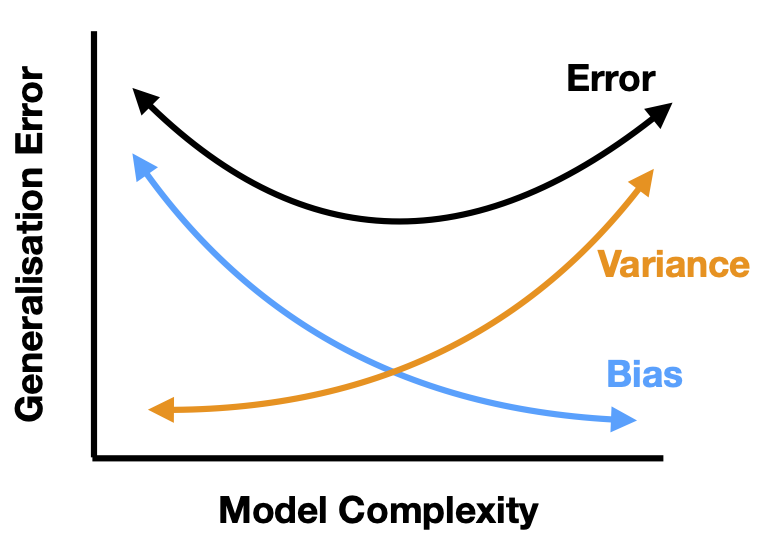
\includegraphics[width=0.5\textwidth]{figures/Bias-Variance-Tradeoff.pdf}
    \caption{\textbf{Schematic depiction of the bias-variance tradeoff.}
    }
\label{fig: Bias-Variance Tradeoff}
\end{figure}

A possible way to reduce generalisation error is actually to drop some data features. From the $n$ data features $\lbrace x_{1}, \dots x_{n} \rbrace$, we can pick a reduced set $\mathcal{M}$. For example, we can choose $\mathcal{M} = \lbrace x_{1}, x_{3}, x_{7} \rbrace$, and define our new linear model as
\begin{equation}\label{eqn: Univariate Subset Linear Model}
    f(\boldsymbol{x}|\bm{\beta}) = \beta_0 + \sum_{j \in \mathcal{M}} \beta_{j}x_{j}.
\end{equation}
This is equivalent to fixing some parameters to zero, i.e., $\beta_k = 0$ if $x_{k} \notin \mathcal{M}$. Minimizing the RSS with this constraint results in a biased estimator but the reduction in model variance can sometimes help to reduce the overall generalisation error. For a small number of features $n \sim 20$, one can search exhaustively for the best subset of features that minimises the error, but beyond that the search becomes computationally unfeasible.

A common alternative is called \emph{ridge regression}\index{ridge regression}. In this method, we consider the same linear model given in Eq.~\eqref{eqn: Univariate Linear Model} but with a modified loss function
\begin{equation}\label{eqn: Ridge}
   % L_{\textrm{ridge}}(\bm{\beta}) = \sum_{i=1}^{m} \left(y_{i} -  \beta_0 +\sum_{j=1}^{n} \beta_{j}x_{ij}\right)^{2} + \lambda \sum_{j=0}^{n} \beta_{j}^{2},
    L_{\textrm{ridge}}(\bm{\beta}) = \sum_{i=1}^{m} \left[y_{i} -   f(\boldsymbol{x}_i|\bm{\beta})\right]^{2} + \lambda \sum_{j=0}^{n} \beta_{j}^{2},
\end{equation}
where $\lambda > 0$ is a positive parameter. 
This is almost the same as the RSS apart from the term proportional to $\lambda$ [c.f. Eq.~\eqref{eqn: RSS}]. The effect of this new term is to penalize large parameters $\beta_j$ and bias the model towards smaller absolute values. The parameter $\lambda$ is an example of a \emph{hyper-parameter}\index{hyper-parameter}, which is kept fixed during the training. On fixing $\lambda$ and minimising the loss function, we obtain the solution
\begin{equation} \label{eqn: Ridge Solution}
    \hat{\bm{\beta}}_{\textrm{ridge}} = (\widetilde{X}^{T}\widetilde{X} + \lambda I)^{-1}\widetilde{X}^{T}\bm{Y},
\end{equation}
from which we can see that as $\lambda \rightarrow \infty$, $\hat{\bm{\beta}}_{\textrm{ridge}} \rightarrow \bm{0}$.
By computing the bias and variance,
\begin{equation}\label{eqn: Ridge Bias-Variance}
    \begin{split}
        \textrm{Bias}(\hat{\bm{\beta}}_{\textrm{ridge}}) &= -\lambda (\widetilde{X}^{T}\widetilde{X} + \lambda I)^{-1} \bm{\beta}^{\textrm{true}}\\
        \textrm{Var}(\hat{\bm{\beta}}_{\textrm{ridge}}) &= \sigma^2 (\widetilde{X}^{T}\widetilde{X} + \lambda I)^{-1} \widetilde{X}^{T}\widetilde{X}(\widetilde{X}^{T}\widetilde{X} + \lambda I)^{-1},
    \end{split}
\end{equation}
it is also obvious that increasing $\lambda$ increases the bias, while reducing the variance. This is the tradeoff between bias and variance. By appropriately choosing $\lambda$ it is possible that generalisation error can be reduced. We will introduce in the next section a common strategy how to find the optimal value for $\lambda$.

The techniques presented here to reduce the generalization error, namely dropping of features and biasing the model to small parameters, are part of a large class of methods known as \emph{regularization}\index{regularization}. Comparing the two methods, we can see a similarity. Both methods actually reduce the complexity of our model. In the former, some parameters are set to zero, while in the latter, there is a constraint which effectively reduces the magnitude of all parameters. A less complex model has a smaller variance but larger bias. By balancing these competing effects, generalisation can be improved, as illustrated schematically in Fig.~\ref{fig: Bias-Variance Tradeoff}.

In the next chapter, we will see that these techniques are useful beyond applications to linear methods. We illustrate the different concepts in the following example.

\begin{figure}[t]
\centering
    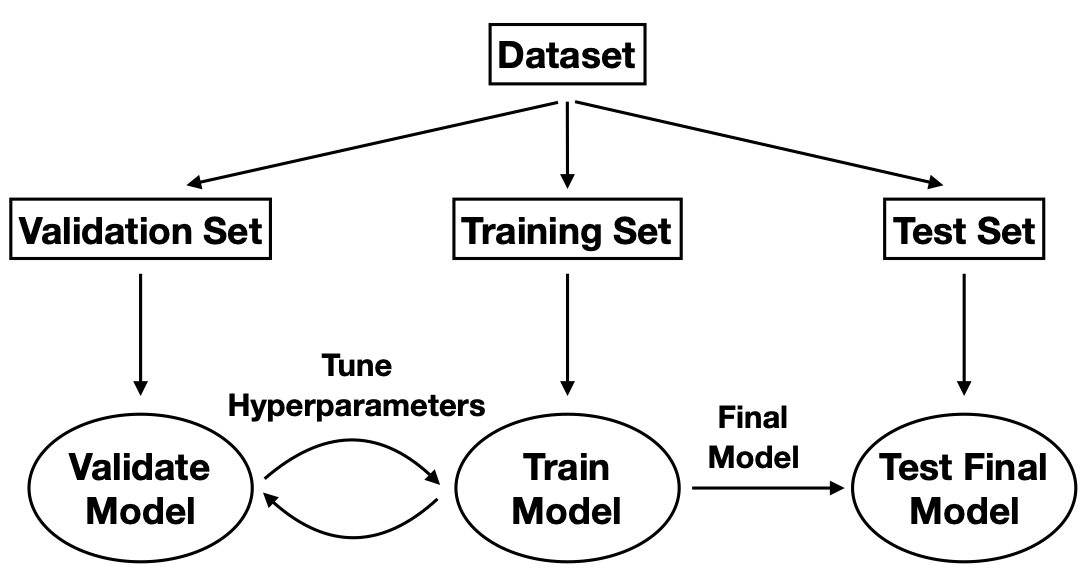
\includegraphics[width=0.7\textwidth]{figures/ML_Workflow.pdf}
    \caption{\textbf{Machine Learning Workflow.}}
\label{fig: ML Workflow}
\end{figure}
\subsubsection{Example}
We illustrate the concepts of linear regression using a medical dataset. In the process, we will also familiarize ourselves with the standard machine learning workflow [see Fig.~\ref{fig: ML Workflow}]. For this example, we are given $10$ data features, namely age, sex, body mass index, average blood pressure, and six blood serum measurements from $442$ diabetes patients, and our task is train a model $f(\bm{x}|\bm{\beta})$ [Eq.~\eqref{eqn: Univariate Linear Model}] to predict a quantitative measure of the disease progression after one year. 

Recall that the final aim of a machine-learning task is not to obtain the smallest possible value for the loss function such as the RSS, but to minimise the generalisation error on unseen data [c.f. Eq.~\eqref{eqn: MSE Generalisation Error}]. The standard approach relies on a division of the dataset into three subsets: training set, validation set and test set. %A common ratio for the split is $70 : 15 : 15$. 
The standard workflow is summarised in Box \ref{box: ML Workflow}.
\begin{mybox}[ML Workflow]{box: ML Workflow}
\begin{enumerate}
    \item Divide the dataset into training set $\mathcal{T}$, validation set $\mathcal{V}$ and test set $\mathcal{S}$. A common ratio for the split is $70 : 15 : 15$.
    \item Pick the hyperparameters, e.g., $\lambda$ in Eq.~\eqref{eqn: Ridge}.
    \item Train the model with only the training set, in other words minimize the loss function on the training set. [This corresponds to Eq.~\eqref{eqn: LG RSS Solution} or \eqref{eqn: Ridge Solution} for the linear regression, where $\widetilde{X}$ only contains the training set.]
    \item Evaluate the MSE (or any other chosen metric) on the validation set, [c.f. Eq.~\eqref{eqn: MSE Generalisation Error}]
    \begin{equation}
        \textrm{MSE}_{\textrm{validation}}(\hat{\bm{\beta}}) = \frac{1}{|\mathcal{V}|}\sum_{j\in\mathcal{V}} (y_j - f(\bm{x}_j|\hat{\bm{\beta}}))^2.
    \end{equation}
This is known as the \emph{validation error}\index{validation error}.
    \item Pick a different value for the hyperparameters and repeat steps $3$ and $4$, until validation error is minimized.
    \item Evaluate the final model on the test set
    \begin{equation}
        \textrm{MSE}_{\textrm{test}}(\hat{\bm{\beta}}) = \frac{1}{|\mathcal{S}|}\sum_{j\in\mathcal{S}} (y_j - f(\bm{x}_j|\hat{\bm{\beta}}))^2.
    \end{equation}
\end{enumerate}
\end{mybox}

It is important to note that the test set $\mathcal{S}$ was not involved in optimizing either parameters $\bm{\beta}$ or the hyperparameters such as $\lambda$.

Applying this procedure to the diabetes dataset\footnote{Source: \href{https://www4.stat.ncsu.edu/~boos/var.select/diabetes.html}{https://www4.stat.ncsu.edu/$\small{\sim}$boos/var.select/diabetes.html}}, we obtain the results in Fig.~\ref{fig: Regression on Diabetes Dataset}. We compare RSS linear regression with the ridge regression, and indeed we see that by appropriately choosing the regularisation hyperparameter $\lambda$, the generalisation error can be minimized.

As side remark regarding the ridge regression, we can see on the left of Fig.~\ref{fig: Ridge Parameters}, that as $\lambda$ increases, the magnitude of the parameters, Eq.~\eqref{eqn: Ridge Solution}, $\hat{\bm{\beta}}_{\textrm{ridge}}$ decreases. Consider on the other hand, a different form of regularisation, which goes by the name \emph{lasso regression}\index{lasso regression}, where the loss function is given by
\begin{equation}\label{eqn: Lasso}
    %L_{\textrm{lasso}}(\bm{\beta}) = \sum_{i=1}^{m} \left(y_{i} -  \beta_0 +\sum_{j=1}^{n} \beta_{j}x_{ij}\right)^{2} + \alpha \sum_{j=0}^{n} |\beta_{j}|.
    L_{\textrm{lasso}}(\bm{\beta}) = \sum_{i=1}^{m} \left[y_{i} -  f(\boldsymbol{x}_i|\bm{\beta})\right]^{2} + \alpha \sum_{j=0}^{n} |\beta_{j}|.
\end{equation}
Despite the similarities, lasso regression has a very different behaviour as depicted on the right of Fig.~\ref{fig: Ridge Parameters}. Notice that as $\alpha$ increases some parameters actually vanish and can be ignored completely. This actually corresponds to dropping certain data features completely and can be useful if we are interested in selecting the most important features in a dataset. 

\begin{figure}[t]
\centering
    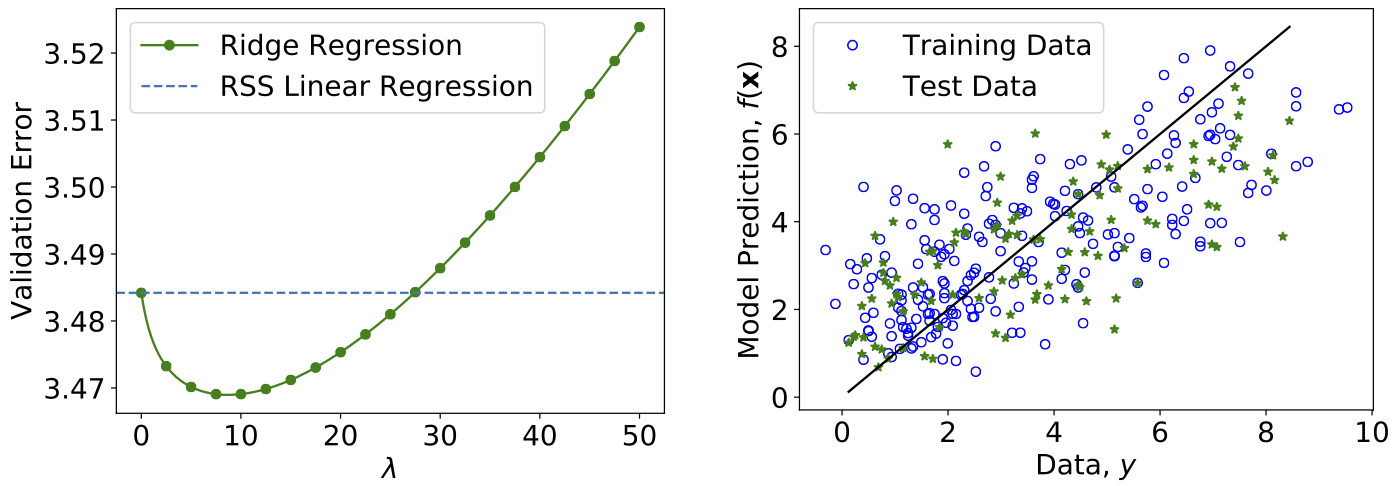
\includegraphics[width=1.0\textwidth]{figures/diabetes_ridge_regression.pdf}
    \caption{\textbf{Ridge Regression on Diabetes patients dataset.} Left: Validation error versus $\lambda$. Right: Test data versus the prediction from the trained model. If 
    the prediction were free of any error, all the points would fall on the blue line.
    }
\label{fig: Regression on Diabetes Dataset}
\end{figure}

\begin{figure}[bh]
\centering
    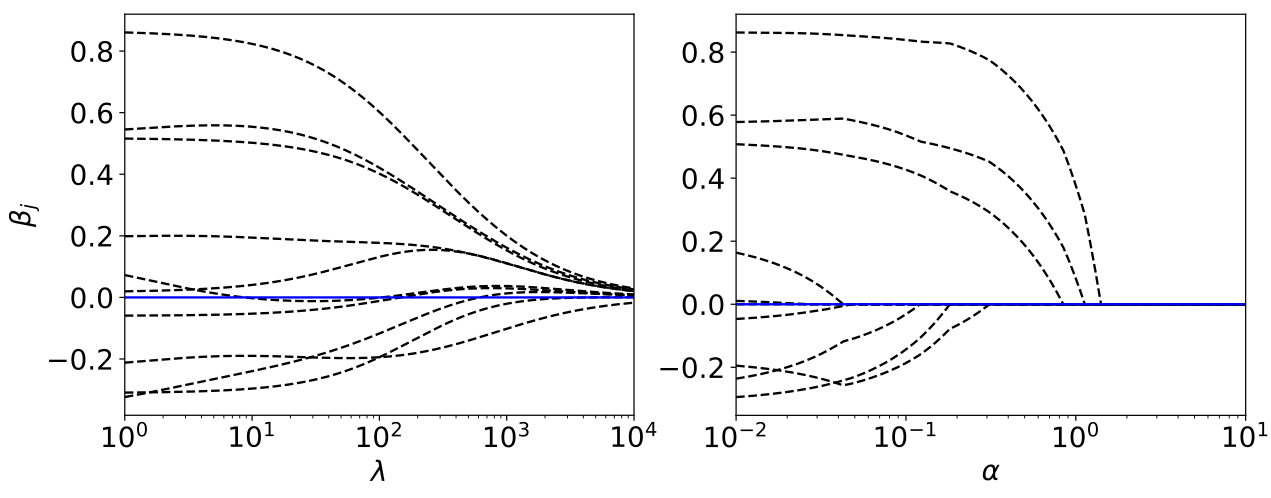
\includegraphics[width=1.0\textwidth]{figures/ridge_variables.pdf}
    \caption{
    \textbf{Evolution of the model parameters.} Increasing the hyperparameter $\lambda$ or $\alpha$ leads to a reduction of the absolute value of the model parameters, here shown for the ridge (left) and Lasso (right) regression for the Diabetes dataset.
    }
\label{fig: Ridge Parameters}
\end{figure}
%
%\subsection{Linear Method for Classification}
%In a classification problem, the aim is to categorise the inputs into one of a finite set of classes. Formulated as a supervised learning task, the dataset again consists of input-output pairs, i.e. $\lbrace(\bm{x}_{1}, y_{1}), \dots, (\bm{x}_{m}, y_{m})\rbrace$. However, unlike regression problems, the output $y$ is a discrete integer number representing one of the classes. 
%
%Suppose we have $p$ classes. Then it seems most natural for the output to take the integer values $y = 1, \dots, p$. However, it turns out to be helpful to use a different, so-called \emph{one-hot encoding}\index{one-hot encoding}. In this encoding, the output $y$ is instead represented by the $p$-dimensional unit vector in $y$ direction $\bm{e}^{(y)}$,
%\begin{equation} \label{eqn: One-Hot Encoding}
%    y \longrightarrow \bm{e}^{(y)} =
%    \begin{bmatrix}
%        e^{(y)}_1 \\
%        \vdots \\
%        e^{(y)}_y \\
%        \vdots \\
%        e^{(y)}_{p}
%    \end{bmatrix}
%    =
%    \begin{bmatrix}
%        0 \\
%        \vdots \\
%        1 \\
%        \vdots \\
%        0
%    \end{bmatrix},
%\end{equation}
%where $e^{(y)}_l = 1$ if $l = y$  and zero for all other $l=1,\ldots, p$. A further advantage of this encoding is that we are not forced to choose a potentially biasing ordering of the classes as we would when arranging them along the ray of integers.
%
%A linear approach to this problem then mirrors the case for linear regression.
%We fit a multi-variate linear model, Eq.~\eqref{eqn: Multivariate Linear Model}, to the one-hot encoded dataset \allowbreak$\lbrace(\bm{x}_{1}, \bm{e}^{(y_1)}), \dots, (\bm{x}_{m}, \bm{e}^{(y_m)})\rbrace$. By minimising the RSS, Eq.~\eqref{eqn: RSS}, we obtain the solution
%\begin{equation}
%    \hat{\bm{\beta}} = (\widetilde{X}^{T}\widetilde{X})^{-1} \widetilde{X}^{T} Y,
%\end{equation}
%where $Y$ is the $m$ by $p$ output matrix. The prediction given an input $\bm{x}$ is then a $p$-dimensional vector $\bm{f}(\bm{x}|\bm{\beta}) = \tilde{\bm{x}}^{T} \hat{\bm{\beta}}$. On a generic input $\bm{x}$, it is obvious that the components of this prediction vector would be real valued, rather than being one of the one-hot basis vectors. To obtain a class prediction $G(\bm{x}|\bm{\beta}) = 1, \dots, p$, we simply take the index of the largest component of that vector, i.e.,
%\begin{equation}
%    F(\bm{x}|\bm{\beta}) = \textrm{argmax}_{k} f_{k}(\bm{x}|\bm{\beta}).
%\end{equation}
%The $\textrm{argmax}$ function is a non-linear function and is a first example of what is referred to as \emph{activation function}\index{activation function}. We will encounter more examples of such activation functions in the next chapter.
%
%The current linear approach based on classification of one-hot encoded data generally works poorly when there are more than two classes. We will see in the next chapter that relatively straightforward non-linear extensions of this approach can lead to much better results.
